\documentclass[a4paper,11pt]{article}
\usepackage{indentfirst}
\setlength\parindent{24pt}
\usepackage[T1]{fontenc}
\usepackage[polish]{babel}
\usepackage[utf8]{inputenc}
\usepackage{lmodern}
\selectlanguage{polish}
\usepackage[top=2cm, bottom=2cm, left=1cm, right=1cm]{geometry}
\usepackage{lastpage}
\usepackage{fancyhdr}
\pagestyle{fancy}
\makeatletter
\newcommand{\linia}{\rule{\linewidth}{0.4mm}}
\renewcommand{\maketitle}{\begin{titlepage}
    \vspace*{2cm}
    \begin{center}\LARGE
    Politechnika Warszawska\\
    Wydział Elektryczny\\
    \end{center}
    \vspace{5cm}
    \noindent\linia
    \begin{center}
      \LARGE \textsc{\@title}
         \end{center}
     \linia
    \vspace{0.5cm}
    \begin{flushright}
    \begin{minipage}{5cm}
    \textit{Autor:}\\
    \normalsize \textsc{\@author} \par
    \end{minipage}
    \vspace{5cm}
     \end{flushright}
    \vspace*{\stretch{6}}
    \begin{center}
    \@date
    \end{center}
  \end{titlepage}
}
\makeatother
\author{Grzegorz Kopyt}
\title{Specyfikacja Implementacyjna \\
,,Arbitrage''}
\usepackage{graphicx}
\fancyhf{}
\rfoot{\thepage{}/\pageref{LastPage}}
\begin{document}

\maketitle

\tableofcontents
\vspace{1cm}
\noindent\linia

\section{Wstęp teoretyczny}
Dokument ten dotyczy implementacji programu ,,Arbitrage". Został przygotowany w celu przedstawienia pomysłu na algorytm realizujący znajdowanie korzystnej ścieżki wymiany walut oraz dowolnego arbitrażu. Ponadto dokument informuje o technologiach, w których program będzie zrealizowany, testach jakie powinny zostać przeprowadzone oraz sprzęcie, na którym zostanie wykonany i uruchomiony.
\section{Diagram klas}
\begin{center}
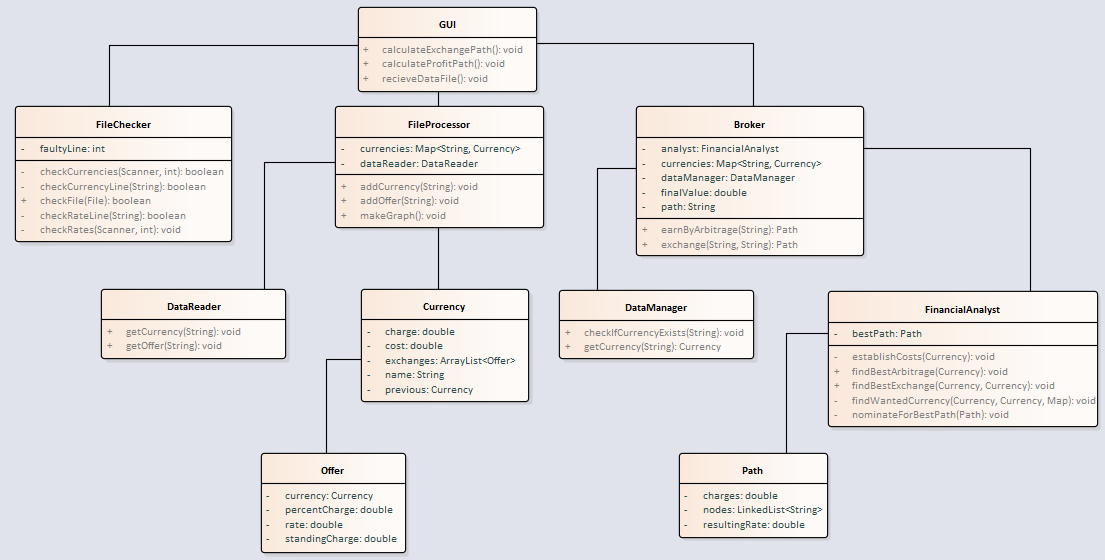
\includegraphics[width = 19cm]{DiagramKlas}
\end{center}

\noindent\linia
\section{Opis algorytmu}

\subsection{Wczytanie danych}

Dane wczytywane będą z pliku tekstowego, wykonanego według wzoru podanym w specyfikacji funkcjonalnej. Plik ten będzie zawierał definicje walut oraz kursy ich wymiany. Na początku zostanie sprawdzony pod kątem zgodności ze wzorem. Jeśli plik będzie wadliwy, algorytm przerwie swoje działanie, a w przeciwnym wypadku będzie kontynuował prace.

Algorytm umieści wszystkie zdefiniowane skrócone nazwy walut w \textit{HashMapie} jako obiekty \textit{Currency}. Dodatkowo każdy obiekt \textit{Currency}, będzie zawierał \textit{Liste} obiektów klasy \textit{Offer}, w których zawarte będą informacje o kosztach i kursie wymiany na inną walutę.
\\Przykład:
\begin{center}
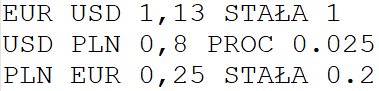
\includegraphics[width = 5cm]{Przyklad}
\end{center}

Obiekt \textit{Currency} reprezentujący walutę \textit{EUR}, będzie zawierał \textit{Liste}, w której będzie obiekt \textit{Offer}.
\\Obiekt \textit{Offer} będzie zawierał:
\begin{itemize}
\item referencję do obiektu \textit{Currency} reprezentującego \textit{USD},
\item informację o kursie wymiany \textit{EUR} na \textit{USD} równym 1.13,
\item informacje o opłacie stałej równej 1,
\item informacje o opłacie procentowej równej 0 (bo jej nie ma w tym przypadku).
\end{itemize} 

Dla innego zestawu danych na tej \textit{Liście} może pojawić się więcej obiektów \textit{Offer} zawierających informacje o~wymianie \textit{EUR} na inne waluty.

W ten sposób obiekty \textit{Currency} i ich \textit{Listy} obiektów \textit{Offer} utworzą graf albo wiele grafów w zależności od danych wejściowych i możliwości wymian między walutami.

Obiekty \textit{Currency} będą węzłami, a obiekty \textit{Offer} czymś na kształt gałęzi jako, że łączą ze sobą węzły.

\subsection{Koszt ścieżki}
Kluczowym zadaniem algorytmu, będzie znajdowanie najkorzystniejszych ścieżek po grafie walut. W wyborze najkorzystniejszej ścieżki pomoże nam koszt ścieżki.
Koszt ścieżki będzie kosztem odwiedzenia danego węzła w zależności od węzła początkowego. W celu określenia kosztu odwiedzenia danego węzła, każdy węzeł będzie przechowywał informacje o koszcie dotarcia do niego.
\\\\Koszt ten będzie składał się z dwóch czynników:
\begin{itemize}
\item kosztu (\textit{cost}) - "kurs" wymiany waluty początkowej na walutę obecnego węzła przez najkorzystniejszą ścieżkę (zawiera opłaty procentowe napotkane na ścieżce),
\item opłaty stałe (\textit{charge}) - w walucie obecnego węzła, wszystkie napotkane na ścieżce.
\end{itemize}
Przykład:

\begin{center}
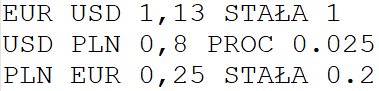
\includegraphics[width = 5cm]{Przyklad}
\end{center}

\begin{enumerate}
\item \textit{Cost} dotarcia do \textit{EUR} oraz jego \textit{charge} będą równe zero, ponieważ od tego węzła zaczniemy.
\item \textit{Cost} dotarcia do \textit{USD} będzie równy 1.13, a jego \textit{charge} będzie równa 1.
\item Następnie:
\begin{enumerate}
\item  \textit{Cost} dotarcia do \textit{PLN} będzie równy \textit{1.13 * 0.8 * (1-0.025) = 0.8814},

		tzn. (\textit{cost USD}) * (kurs wymiany \textit{USD} na \textit{PLN}) * (1 - opłata procentowa).
\item \textit{Charge} dotarcia do \textit{PLN} będzie równa \textit{1 * 0.8 + 0 = 0.8},

		tzn. (\textit{charge USD}) *  (kurs wymiany \textit{USD} na \textit{PLN}) + opłata stała.
\end{enumerate}
\item Następnie:
\begin{enumerate}
\item  \textit{Cost} dotarcia do \textit{EUR} będzie równy \textit{0.8814 * 0.25 * (1-0) = 0.22035},

		tzn. (\textit{cost PLN}) * (kurs wymiany \textit{PLN} na \textit{EUR}) * (1 - opłata procentowa).
\item \textit{Charge} dotarcia do \textit{EUR} będzie równa \textit{0.8 * 0.25 + 0.2 = 0.4},

		tzn. (\textit{charge PLN}) *  (kurs wymiany \textit{PLN} na \textit{EUR}) + opłata stała.
\end{enumerate}
\end{enumerate}

Kiedy wszystkie węzły otrzymają swój najkorzystniejszy koszt ( o czym w dalszej części specyfikacji), wtedy wartości tych kosztów mogą posłużyć do obliczenia kwoty końcowej, jaką użytkownik uzyska z wymiany walut.
\\Przykład:
\begin{enumerate}
\item Węzłem początkowym było \textit{EUR}.
\item 1000 \textit{EUR} chcemy wymienić na \textit{PLN}.
\item Sprawdzamy koszt \textit{PLN}:
\begin{itemize}
\item \textit{cost} wynosi 0.8814,
\item \textit{charge} wynosi 0.8 (w \textit{PLN}, dlatego trzeba przeliczyć na \textit{EUR}).
\end{itemize}
\item Z wymiany uzyskamy kwotę \textit{(1000 * 0.8814) - (0.8 / 0.8814) = 880.49},

		tzn. kwota * (\textit{cost PLN}) - (\textit{charge / cost PLN}).
\end{enumerate}

Z powyższego przykładu wynika, że najkorzystniejsza ścieżka to taka, której \textit{cost} jest jak największy, a \textit{charge} jak najmniejsza. Łatwo zauważyć, że opłacalność ścieżki w dużej mierze zależy od kwoty, którą dysponujemy. Przykładowo, jeśli chcemy wymienić 1 \textit{EUR} i otrzymamy 100 \textit{PLN}, a~opłata wynosi 100~\textit{PLN}, to nie opłaca nam się zupełnie taka transakcja. Natomiast w przypadku, gdy wymieniamy 1000~\textit{EUR} i otrzymamy 100 000~\textit{PLN} to wtedy opłata 100~\textit{PLN} nie robi nam różnicy, dlatego:
\begin{itemize}
\item w przypadku znajdowania najkorzystniejszej ścieżki wymiany waluty (nie znając kwoty wyjściowej), za najkorzystniejszą ścieżkę uznam tę, której \textit{cost} jest największy,
\item w przypadku znajdowania dowolnego arbitrażu (znając kwotę wyjściową), algorytm uwzględni \textit{charge} (o~czym w dalszej części specyfikacji).
\end{itemize}

\subsection{Nadawanie węzłom kosztów}
Algorytm chodzenia po grafie i nadawania węzłom kosztów, będzie oparty o algorytm Bellmana-Forda. Na potrzeby śledzenia ścieżek wymian, obiekty \textit{Currency} będą zawierać pole \textit{previous} z referencją do waluty, która jako ostatnia zmodyfikowała koszt tego węzła (o czym w dalszej części specyfikacji). Nadawanie węzłom kosztów będzie różniło się w zależności od zadania realizowanego przez program (znajdowanie korzystnej ścieżki wymiany waluty lub znajdowanie dowolnego arbitrażu).

\subsubsection{Znajdowanie korzystnej ścieżki wymiany waluty}
Koszty ścieżek dotarcia do danego węzła z węzła początkowego, są ściśle zależne od węzła początkowego. Z tego powodu w klasie \textit{FinancialAnalyst} (odpowiedzialnej za szukanie korzystnej ścieżki wymiany waluty oraz dowolnego arbitrażu) znajdzie się zmienna \textit{graphConfiguration}, która będzie informować o tym na jaki węzeł początkowy skonfigurowany (węzłom nadane są najkorzystniejsze koszty) jest obecnie graf. Pozwoli to w niektórych przypadkach na wykorzystanie pracy, którą program wykonał już wcześniej i nie będzie konieczności wykonywania poniższych instrukcji jeszcze raz.

W przeciwnym wypadku, jeśli graf nie jest jeszcze skonfigurowany albo skonfigurowano go na inny węzeł niż ten obecnie podany przez użytkownika jako waluta wyjściowa, algorytm wykonuje następujące operacje:
\begin{enumerate}
\item Algorytm bierze wszystkie waluty z \textit{HashMapy} i wstawia je do \textit{ArrayListy} (będzie po nich kolejno iterował w obiegu zamkniętym, czyli jak dotrze do końca \textit{Listy}, następnym elementem jest zerowy, potem pierwszy itd.).

		Na początku wartości \textit{cost} i \textit{charge} wszystkich węzłów są ustawiane na liczbę ujemną, a \textit{previous} na wartość \textit{null}.
\item Pierwszą walutą ( węzeł początkowy), od której algorytm rozpocznie nadawanie kosztów, jest ta podana przez użytkownika jako waluta, którą użytkownik chce wymienić,

		Wartości \textit{cost} i \textit{charge} węzła początkowego przyjmują wartość zero.
\item Obecny węzeł (obecna waluta) to waluta początkowa.
\item Flaga zmiany kosztu, która znajdować się będzie w metodzie realizującej to zadanie, zostaje wygaszona, jeśli obecny węzeł to węzeł początkowy.

Flaga zostaje zapalona w momencie kiedy wartość kosztu sąsiadującego węzła zostaje zmodyfikowana.
\item Następnie algorytm nadaje węzłom sąsiadującym z obecnym węzłem koszty w sposób opisany w podsekcji \textit{Koszt ścieżki}, pod warunkiem, że nowy \textit{cost} jest większy od bieżącego znajdującego się w sąsiadującym węźle.

Jeśli ten warunek jest spełniony, w sąsiadującym węźle nadane zostają nowe wartości \textit{cost} oraz \textit{charge}, a~także polu \textit{previous} przypisana zostaje obecna waluta ( ponieważ to ona spowodowała, że nowy \textit{cost} jest większy od starego).

Węzeł początkowy może nadać wartości swoim węzłom sąsiadującym tylko raz. W kolejnych iteracjach pomijamy go, żeby nie wpaść w nieskończoną pętlę.
\item Po zaktualizowaniu kosztów w węzłach sąsiadujących z obecnym węzłem, obecnym węzłem staje się następna waluta według kolejności opisanej w punkcie pierwszym.
\begin{enumerate}
\item Jeśli obecny węzeł jest węzłem początkowym, a flaga zmiany kosztu jest wygaszona, to znaczy, że w~poprzedniej iteracji (jedna iteracja to rozpatrzenie każdego węzła z \textit{ArrayListy} z punktu pierwszego) nie dokonano już żadnej zmiany, czyli nadano już najkorzystniejsze koszty wszystkim węzłom. Zatem korzystna ścieżka wymiany zostaje wyświetlona (o czym w dalszej części specyfikacji).
\item Jeśli obecny węzeł jest węzłem początkowym, a flaga zmiany kosztu jest zapalona, to należy powtórzyć punkty 4-6, ponieważ jeszcze nie nadano najkorzystniejszych kosztów wszystkim węzłom.
\item Jeśli w obecnym węźle wartości \textit{cost} i \textit{charge} są liczbami ujemnymi, a \textit{previous} ma wartość \textit{null}, to znaczy, że jeszcze nie wiemy jak dotrzeć do tego węzła i bez aktualizacji kosztów węzłów sąsiadujących z obecnym węzłem powtarzamy punkt 6.
\item W pozostałym wypadku (różnym od a, b i c) powtarzamy punkty 5-6.
\end{enumerate}
\end{enumerate}

\subsubsection{Znajdowanie dowolnego arbitrażu}
W przypadku znajdowania dowolnego arbitrażu, przy wyszukiwaniu ścieżki takiego arbitrażu brana jest pod uwagę, także \textit{charge} każdego węzła.
W tym celu obiekty \textit{Currency} będą zawierały pole \textit{exchangedMoney}, które przedstawiać będzie kwotę w walucie danego węzła, jaką możemy uzyskać dokonując wymiany kwoty w walucie początkowej na walutę danego węzła po korzystnej ścieżce.
\\Wyszukiwanie arbitrażu działa następująco:
\begin{enumerate}
\item  Algorytm bierze wszystkie waluty z \textit{HashMapy} i wstawia je do \textit{ArrayListy} (będzie po nich kolejno iterował w obiegu zamkniętym, czyli jak dotrze do końca \textit{Listy}, następnym elementem jest zerowy, potem pierwszy itd.).
\item Na początku wartości \textit{cost}, \textit{charge} oraz \textit{exchangedMoney} wszystkich węzłów są ustawiane na liczbę ujemną, a \textit{previous} na wartość \textit{null}.
\item Pierwszą walutą ( węzeł początkowy), od której algorytm rozpocznie nadawanie kosztów, jest ta, która na \textit{Liście} z punktu pierwszego, ma indeks zerowy.

		Wartości \textit{cost} oraz \textit{charge} węzła początkowego przyjmują wartość zero. Wartość \textit{exchangedMoney} zostaje zainicjowana kwotą podaną przez użytkownika.
\item Obecny węzeł (obecna waluta) to waluta początkowa.
\item Flaga zmiany kosztu, która znajdować się będzie w metodzie realizującej to zadanie, zostaje wygaszona, jeśli obecny węzeł to węzeł początkowy.

Flaga zostaje zapalona w momencie kiedy wartość kosztu sąsiadującego węzła zostaje zmodyfikowana.
\item Następnie algorytm nadaje węzłom sąsiadującym z obecnym węzłem koszty w sposób opisany w podsekcji \textit{Koszt ścieżki}, pod warunkiem, że kwota końcowa, (obliczona według wzorca z podsekcji \textit{Koszt ścieżki},  na bazie nowych wartości \textit{cost}, \textit{charge} oraz wartości \textit{exchangedMoney} z obecnego węzła) jest większa od bieżącej wartości \textit{exchangedMoney} znajdującej się w sąsiadującym węźle.

Jeśli ten warunek jest spełniony, w sąsiadującym węźle nadane zostają nowe wartości \textit{cost} oraz \textit{charge}, a~także polu \textit{previous} przypisana zostaje obecna waluta ( ponieważ to ona spowodowała, że nowa wartość \textit{exchangedMoney} jest większa od starej). Pole \textit{exchangedMoney} otrzymuje wartość obliczonej kwoty końcowej.

Węzeł początkowy może nadać wartości swoim węzłom sąsiadującym tylko raz. W kolejnych iteracjach pomijamy go, żeby nie wpaść w nieskończoną pętlę.
\item Po zaktualizowaniu kosztów w węzłach sąsiadujących z obecnym węzłem, obecnym węzłem staje się następna waluta według kolejności opisanej w punkcie pierwszym.
\begin{enumerate}
\item Jeśli obecny węzeł jest węzłem początkowym, a flaga zmiany kosztu jest wygaszona, to znaczy, że w~poprzedniej iteracji (jedna iteracja to rozpatrzenie każdego węzła z \textit{ArrayListy} z punktu pierwszego) nie dokonano już żadnej zmiany, czyli nadano już najkorzystniejsze koszty wszystkim węzłom.
\begin{itemize}
\item Jeżeli wartość \textit{exchangedMoney} obecnego węzła (węzła początkowego) jest większa od wartości podanej przez użytkownika to znaleziono korzystny arbitraż i można wyświetlić jego ścieżkę (o~czym w dalszej części specyfikacji) oraz kwotę.
\item Jeżeli wartość \textit{exchangedMoney} obecnego węzła (węzła początkowego) nie jest większa od wartości podanej przez użytkownika to należy powtórzyć punkty 2-7 z tą różnicą, że w punkcie 3 wartością początkową staje się waluta o indeksie o 1 większym niż obecna (w ArrayLiście z punktu pierwszego).
\item Jeżeli wartość \textit{exchangedMoney} obecnego węzła (węzła początkowego) nie jest większa od wartości podanej przez użytkownika i jest ostatnią waluta na \textit{ArrayLiście}, oznacza to, że dla otrzymanych danych nie można znaleźć arbitrażu. Komunikat o tym zostaje wyświetlony.
\end{itemize}
\item Jeśli obecny węzeł jest węzłem początkowym, a flaga zmiany kosztu jest zapalona, to należy powtórzyć punkty 5-7, ponieważ jeszcze nie nadano najkorzystniejszych kosztów wszystkim węzłom.
\item Jeśli w obecnym węźle wartości \textit{cost} i \textit{charge} są liczbami ujemnymi, a \textit{previous} ma wartość \textit{null}, to znaczy, że jeszcze nie wiemy jak dotrzeć do tego węzła i bez aktualizacji kosztów węzłów sąsiadujących z obecnym węzłem powtarzamy punkt 7.
\item W pozostałym wypadku (różnym od a, b, c i d) powtarzamy punkty 6-7.
\end{enumerate}
\end{enumerate}

\subsubsection{Wyświetlanie ścieżki}
Informacje o elementach szukanej ścieżki znajdują się w polach \textit{previous} obiektów \textit{Currency}.
Napis zawierający cała ścieżkę tworzy się dzięki przechodzenie grafu szlakiem referencji do walut zawartych w polach \textit{previous}:
\begin{itemize}
\item w przypadku znalezienia korzystnej wymiany walut należy rozpocząć od waluty docelowej i podążać kolejno referencjami z pól \textit{previous}, odkładając na stos kolejne nazwy walut, aż dotrzemy do waluty początkowej,
\item w przypadku znalezienia dowolnego arbitrażu, należy rozpocząć od waluty, która została odkryta jako możliwość arbitrażu, a następnie podążając kolejno referencjami z pól \textit{previous}, odkładać na stos kolejne nazwy walut, aż dotrzemy z powrotem do danej waluty.
\end{itemize}

Po tych operacjach należy pobierając ze stosu nazwy walut stworzyć napis reprezentujący korzystną ścieżkę wymiany walut lub arbitraż.
Do realizacji tego zadania przeznaczona jest klasa \textit{Path}, która będzie zawierać potrzebne metody, a także będzie zwracana przez metody odpowiedzialne za znajdowanie korzystnej ścieżki wymiany waluty oraz znajdowanie dowolnego arbitrażu.
Uzyskana ścieżka nie może być krótsza niż dwa węzły.

Ścieżka wyświetlana będzie zgodnie ze specyfikacja funkcjonalną.

\noindent\linia
\section{Opis ważniejszych metod}
\begin{itemize}
\item Path \textbf{findExchange}( waluta początkowa, waluta docelowa)
\\\\
Metoda wykonuje działania opisane w części 3.3.1 tego dokumentu.
\item Path \textbf{findArbitrage}( kwota)
\\\\
Metoda wykonuje działania opisane w części 3.3.2 tego dokumentu.
\item String \textbf{makePath}( stos walut)
\\\\
Metoda wykonuje działania opisane w ostatnim akapicie części 3.3.3 tego dokumentu.
\item String \textbf{checkCurrencyLine}( linia tekstu)
\\\\
Metoda sprawdza czy otrzymana linia jest zgodna ze wzorem. W tym przypadku czy jest to linia przedstawiająca definicje waluty w pliku.

Podobnie działają pozostałe metody z klasy \textit{FileChecker}.
\item String \textbf{addCurrency}( linia tekstu)
\\\\
Metoda, na podstawie linii tekstu z pliku, dodaje do \textit{HashMapy} walutę.
\item String \textbf{addOffer}(  linia tekstu)
\\\\
Metoda, na podstawie linii tekstu z pliku, dodaje do \textit{ArrayListy}, w obiekcie \textit{Currency} reprezentującym odpowiednią walutę, informacje, zawartą w obiekcie  \textit{Offer}, o możliwości wymiany tej waluty na inną.

\end{itemize}

\noindent\linia

\section{Testy}
\begin{itemize}
\item Path \textbf{findExchange}( waluta początkowa, waluta docelowa)
\begin{itemize}
\item Jedna z podanych walut nie istnieje (nie ma jej wśród danych),
\item nie istnieje ścieżka pomiędzy tymi walutami,
\item jedną z podanych wartości jest \textit{null},
\item istnieją obie podane waluty,
\item istnieje ścieżka między podanymi walutami.
\end{itemize}
\item Path \textbf{findArbitrage}( kwota)
\begin{itemize}
\item Kwota jest ujemna,
\item kwota jest równa zero,
\item nie istnieje możliwość arbitrażu,
\item istnieje możliwość arbitrażu.
\end{itemize}
\item String \textbf{makePath}( stos walut)
\begin{itemize}
\item Podano \textit{null},
\item na stosie nic nie ma,
\item na stosie jest jedna waluta,
\item na stosie są dwie waluty.
\end{itemize}
\item String \textbf{checkCurrencyLine}( linia tekstu)
\begin{itemize}
\item Podano \textit{null},
\item podano linię tekstu zgodną ze wzorem,
\item podano linię tekstu niezgodną ze wzorem.
\end{itemize}
\item String \textbf{addCurrency}( linia tekstu)
\begin{itemize}
\item Podano \textit{null},
\item podano linię tekstu zgodną ze wzorem,
\item podano linię tekstu niezgodną ze wzorem,
\item już jest taka waluta w \textit{HashMapie},
\item jeszcze nie ma takiej waluty w \textit{HashMapie}.
\end{itemize}
\item String \textbf{addOffer}(  linia tekstu)
\begin{itemize}
\item Podano \textit{null},
\item podano linię tekstu zgodną ze wzorem,
\item podano linię tekstu niezgodną ze wzorem,
\item już jest taka oferta w \textit{Liście},
\item jeszcze nie ma takiej oferty w \textit{Liście}.
\end{itemize}
\end{itemize}

\noindent\linia
\section{Informacje o sprzęcie i oprogramowaniu}
Program będzie pisany w języku JAVA ( wersja 9.0.4) z wykorzystaniem JavaFX. Zostanie przetestowany na komputerze Lenovo G510 o procesorze Intel Core i5 2.5GHz, pamięci RAM 6GB, karcie graficznej AMD Radeon HD 8570M i~systemie operacyjnym Windows 10.

\noindent\linia

\end{document}



